\chapter{Дизайн и блоковата схема на робота}

\section{Дизайн и Функционални изисквания към робота}
\label{sec:requirements}

В рамките на дипломната работа бойният робот, който се разработва, е с оръжие "hammer saw". Този вид оръжие е хибрид между пневматичните чукове и въртящите се режещи дискове. По дизайн оръжието е диск, чиято формата не е перфектен кръг, а е неправилна особена форма. Тя може да бъде видяна на \cref{fig:disk}. Разработения робот е вдъхновен от робота SawBlaze участник от телевизионното състезание BattleBots.

\begin{figure}[H]
    \centering
    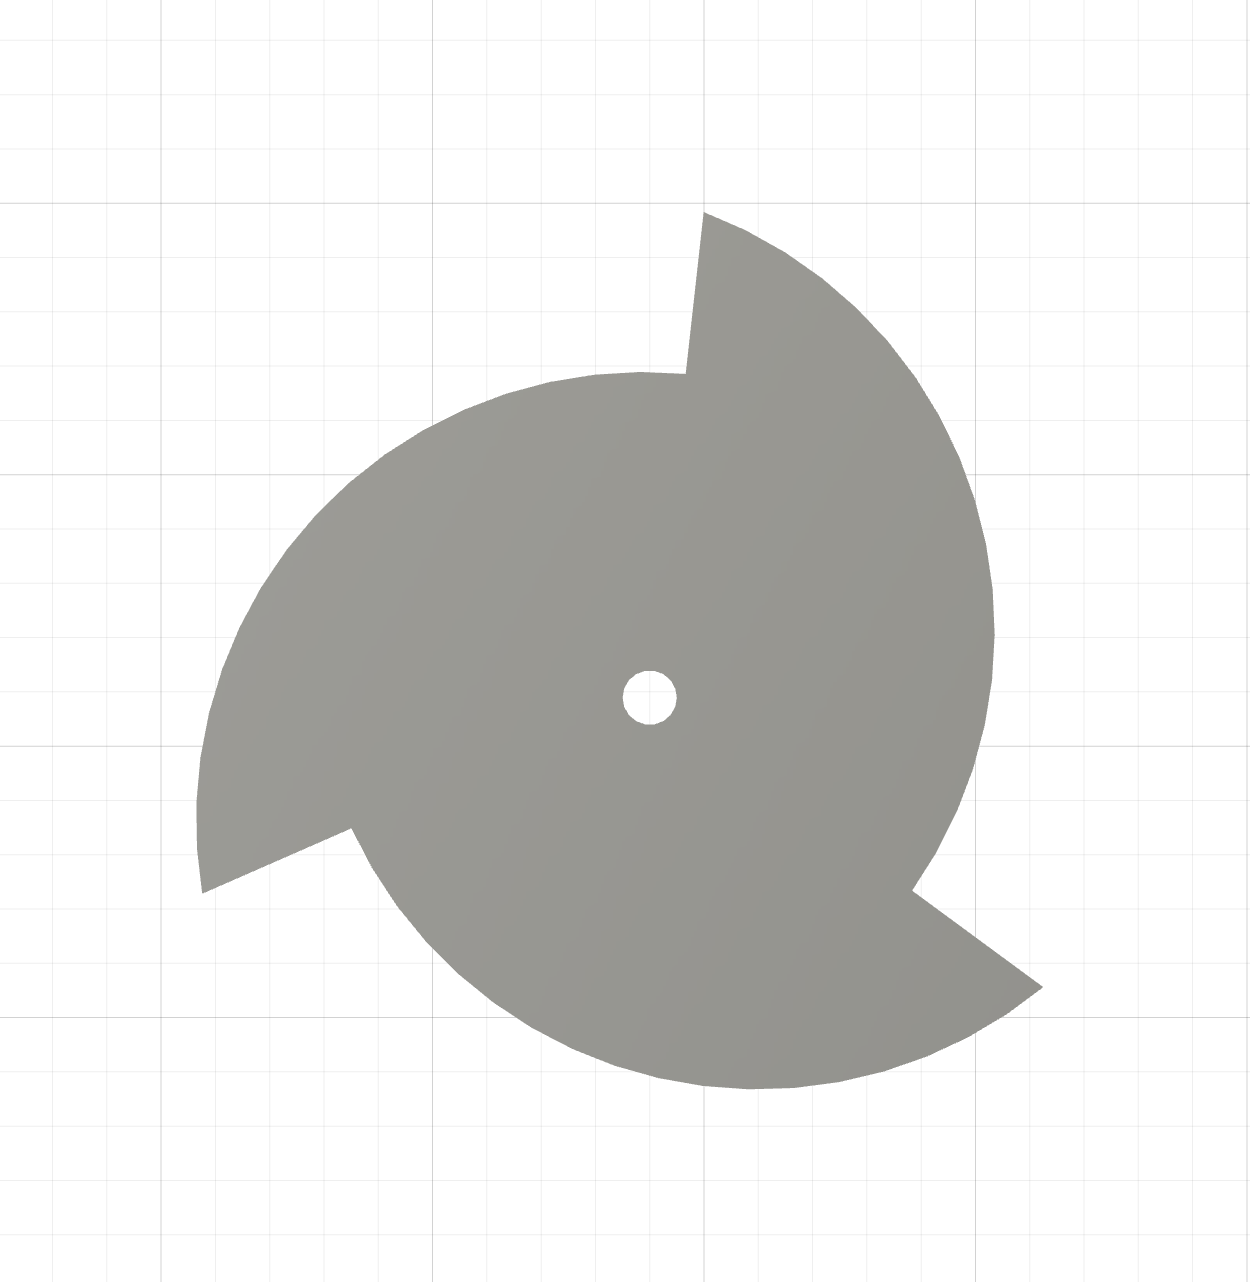
\includegraphics[width=0.6\linewidth]{images/disk.png}
    
    \caption{Хоризонтален разрез на оръжието}
    \label{fig:disk} 
\end{figure}


\section{Блок схеми}
\label{sec:block-schemas}

На \cref{fig:block-controller} и \cref{fig:block-robot} са представени блоковите схеми на пулта за управление и робота. Със син цвят са представени устройствата слаботоковите устройства, а червен захранването и силовата електроника. Черните стрелки на схемите представляват пренос на данни, а червените - захранване.

Основния компонент в схемата на дистанционното печатната платка, върху която седи микроконтролерът и радиочестотния модул. Това което микроконтролера прави е да прочита данните от бутоните и потенциометрите и да се предават посредством радио модула до печатната платка в робота. За повече информация какъв е цикъла на работа може да се прочете \cref{sec:logic-schemas}.

\begin{figure}[H]
    \centering
    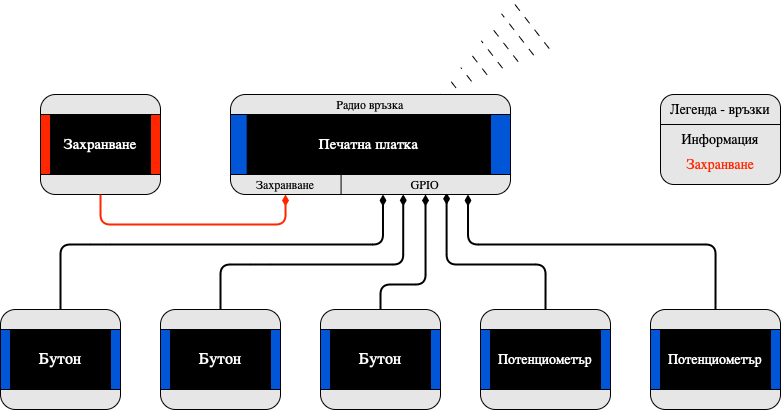
\includegraphics[width=\linewidth]{images/block-schema-controller.png}
    
    \caption{Блокова схема на дистанционното}
    \label{fig:block-controller} 
\end{figure}

Подобно на пулта за управление основния компонент в робота е печатната платка, защото на нея са поставени избраният микроконтролер и радиочестотния модул. Тук функцията на nRF модула е да се получават данните изпратени от дистанционното и да се предадат на микроконтролера. Той на свой ред ги изпълнява като в зависимост от тях се променя управлението на силовите компоненти. Два от четковите мотори се използват за задвижване на робота, а третия за завъртане на оръжието. Стъпковият мотор се използва за да се контролира позицията на ръката с оръжието. Успоредно на това чрез оптичните сензори се следи скоростта на четковите мотори. Освен това чрез крайните изключватели се следи стъпковия мотор да не излиза извън крайните си състояния.

\begin{figure}[H]
    \centering
    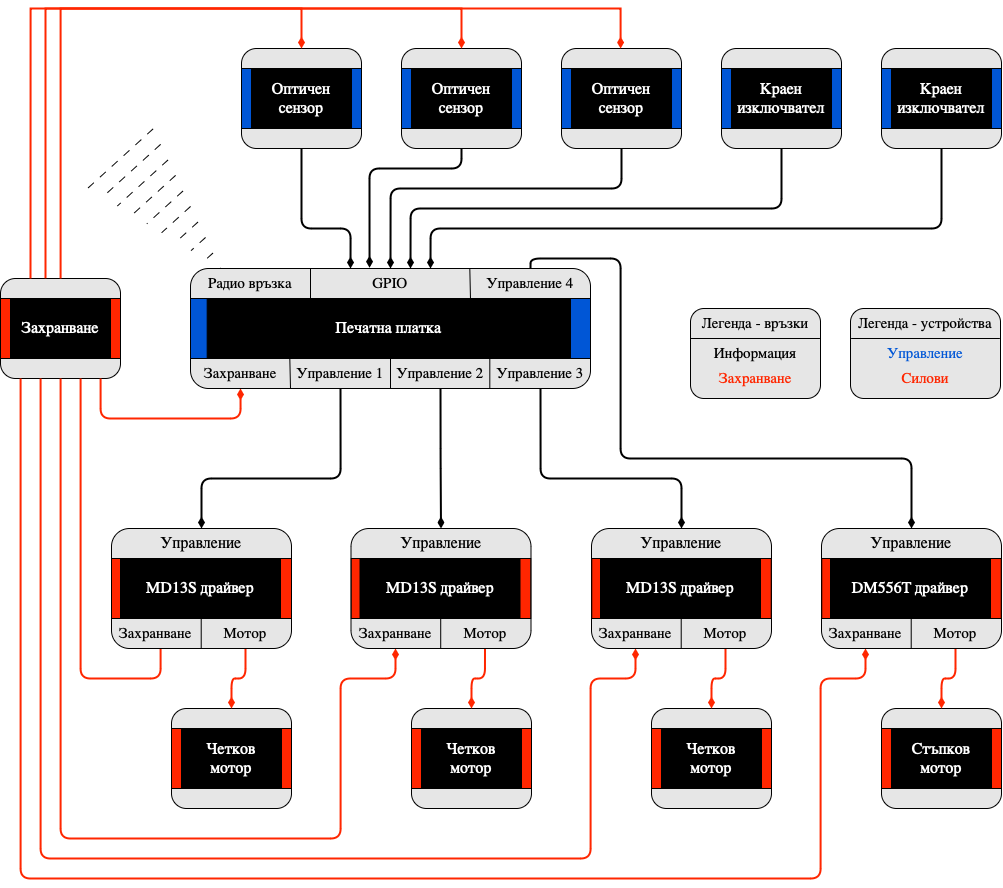
\includegraphics[width=\linewidth]{images/block-schema-robot.png}
    
    \caption{Блокова схема на робота}
    \label{fig:block-robot} 
\end{figure}